\documentclass[12pt,spanish,fleqn,openany,letterpaper,pagesize]{scrbook}

\usepackage[utf8]{inputenc}
\usepackage[spanish]{babel}
\usepackage{fancyhdr}
\usepackage{epsfig}
\usepackage{epic}
\usepackage{eepic}
\usepackage{amsmath}
\usepackage{threeparttable}
\usepackage{amscd}
\usepackage{here}
\usepackage{graphicx}
\usepackage{lscape}
\usepackage{tabularx}
\usepackage{subfigure}
\usepackage{longtable}


\usepackage{rotating} %Para rotar texto, objetos y tablas seite. No se ve en DVI solo en PS. Seite 328 Hundebuch
                        %se usa junto con \rotate, \sidewidestable ....


\renewcommand{\theequation}{\thechapter-\arabic{equation}}
\renewcommand{\thefigure}{\textbf{\thechapter-\arabic{figure}}}
\renewcommand{\thetable}{\textbf{\thechapter-\arabic{table}}}


\pagestyle{fancyplain}%\addtolength{\headwidth}{\marginparwidth}
\textheight22.5cm \topmargin0cm \textwidth16.5cm
\oddsidemargin0.5cm \evensidemargin-0.5cm%
\renewcommand{\chaptermark}[1]{\markboth{\thechapter\; #1}{}}
\renewcommand{\sectionmark}[1]{\markright{\thesection\; #1}}
\lhead[\fancyplain{}{\thepage}]{\fancyplain{}{\rightmark}}
\rhead[\fancyplain{}{\leftmark}]{\fancyplain{}{\thepage}}
\fancyfoot{}
\thispagestyle{fancy}%


\addtolength{\headwidth}{0cm}
\unitlength 1mm %Define la unidad LE para Figuras
\mathindent 1cm %Define la distancia de las formulas al texto,  fleqn las descentra
\marginparwidth 0cm
\parindent 0.5cm %Define la distancia de la primera linea de un parrafo a la margen

%Para tablas,  redefine el backschlash en tablas donde se define la posici\'{o}n del texto en las
%casillas (con \centering \raggedright o \raggedleft)
\newcommand{\PreserveBackslash}[1]{\let\temp=\\#1\let\\=\temp}
\let\PBS=\PreserveBackslash

%Espacio entre lineas
\renewcommand{\baselinestretch}{1.1}

%Neuer Befehl f\"{u}r die Tabelle Eigenschaften der Aktivkohlen
\newcommand{\arr}[1]{\raisebox{1.5ex}[0cm][0cm]{#1}}

%Neue Kommandos
\usepackage{Befehle}


%Trennungsliste
\hyphenation {Reaktor-ab-me-ssun-gen Gas-zu-sa-mmen-set-zung
Raum-gesch-win-dig-keit Durch-fluss Stick-stoff-gemisch
Ad-sorp-tions-tem-pe-ra-tur Klein-schmidt
Kohlen-stoff-Mole-kular-siebe Py-rolysat-aus-beu-te
Trans-port-vor-gan-ge}

% Comandos propios
\newcommand{\surr}[2]{\{#1\;|\;#2\}}
%\includeonly{Kap1/Kap1,Kap2/Kap2}
\begin{document}
\pagenumbering{roman}
%\newpage
%\setcounter{page}{1}
\begin{center}
\begin{figure}
\centering%

\epsfig{file=HojaTitulo/EscudoUN.eps,scale=1}%
\end{figure}
\thispagestyle{empty} \vspace*{2.0cm} \textbf{\huge
T\'{\i}tulo de la tesis  o trabajo de investigaci\'{o}n}\\[6.0cm]
\Large\textbf{Nombres y apellidos completos del autor}\\[6.0cm]
\small Universidad Nacional de Colombia\\
Facultad, Departamento (Escuela, etc.)\\
Ciudad, Colombia\\
A\~{n}o\\
\end{center}

\newpage{\pagestyle{empty}\cleardoublepage}

\newpage
\begin{center}
\thispagestyle{empty} \vspace*{0cm} \textbf{\huge
T\'{\i}tulo de la tesis  o trabajo de investigaci\'{o}n}\\[3.0cm]
\Large\textbf{Nombres y apellidos completos del autor}\\[3.0cm]
\small Tesis o trabajo de grado presentada(o) como requisito parcial para optar al
t\'{\i}tulo de:\\
\textbf{Indicar el t\'{\i}tulo que se obtendr\'{a}. Por ejemplo, Magister en Ingenier\'{\i}a Qu\'{\i}mica}\\[2.5cm]
Director(a):\\
T\'{\i}tulo (Ph.D., Doctor, Qu\'{\i}mico, etc.) y nombre del director(a)\\[2.0cm]
L\'{\i}nea de Investigaci\'{o}n:\\
Nombrar la l\'{\i}nea de investigaci\'{o}n en la que enmarca la tesis  o trabajo de investigaci\'{o}n\\
Grupo de Investigaci\'{o}n:\\
Nombrar el grupo en caso que sea posible\\[2.5cm]
Universidad Nacional de Colombia\\
Facultad, Departamento (Escuela, etc.)\\
Ciudad, Colombia\\
A\~{n}o\\
\end{center}

\newpage{\pagestyle{empty}\cleardoublepage}

\newpage
\thispagestyle{empty} \textbf{}\normalsize
\\\\\\%
\textbf{(Dedicatoria o un lema)}\\[4.0cm]

\begin{flushright}
\begin{minipage}{8cm}
    \noindent
        \small
        Su uso es opcional y cada autor podr\'{a} determinar la distribuci\'{o}n del texto en la p\'{a}gina, se sugiere esta presentaci\'{o}n. En ella el autor dedica su trabajo en forma especial a personas y/o entidades.\\[1.0cm]\\
        Por ejemplo:\\[1.0cm]
        A mis padres\\[1.0cm]\\
        o\\[1.0cm]
        La preocupaci\'{o}n por el hombre y su destino siempre debe ser el
        inter\'{e}s primordial de todo esfuerzo t\'{e}cnico. Nunca olvides esto
        entre tus diagramas y ecuaciones.\\\\
        Albert Einstein\\
\end{minipage}
\end{flushright}

\newpage{\pagestyle{empty}\cleardoublepage}

\newpage
\thispagestyle{empty} \textbf{}\normalsize
\\\\\\%
\textbf{\LARGE Agradecimientos}
\addcontentsline{toc}{chapter}{\numberline{}Agradecimientos}\\\\
Esta secci\'{o}n es opcional, en ella el autor agradece a las personas o instituciones que colaboraron en la realizaci\'{o}n de la tesis  o trabajo de investigaci\'{o}n. Si se incluye esta secci\'{o}n, deben aparecer los nombres completos, los cargos y su aporte al documento.\\

\newpage{\pagestyle{empty}\cleardoublepage}

\newpage
\textbf{\LARGE Resumen}
\addcontentsline{toc}{chapter}{\numberline{}Resumen}\\\\
El resumen es una presentaci\'{o}n abreviada y precisa (la NTC 1486 de 2008 recomienda revisar la norma ISO 214 de 1976). Se debe usar una extensi\'{o}n m\'{a}xima de 12 renglones. Se recomienda que este resumen sea anal\'{\i}tico, es decir, que sea completo, con informaci\'{o}n cuantitativa y cualitativa, generalmente incluyendo los siguientes aspectos: objetivos, dise\~{n}o, lugar y circunstancias, pacientes (u objetivo del estudio), intervenci\'{o}n, mediciones y principales resultados, y conclusiones. Al final del resumen se deben usar palabras claves tomadas del texto (m\'{\i}nimo 3 y m\'{a}ximo 7 palabras), las cuales permiten la recuperaci\'{o}n de la informaci\'{o}n.\\

\textbf{\small Palabras clave: (m\'{a}ximo 10 palabras, preferiblemente seleccionadas de las listas internacionales que permitan el indizado cruzado)}.\\

A continuaci\'{o}n se presentan algunos ejemplos de tesauros que se pueden consultar para asignar las palabras clave, seg\'{u}n el \'{a}rea tem\'{a}tica:\\

\textbf{Artes}: AAT: Art y Architecture Thesaurus.

\textbf{Ciencias agropecuarias}: 1) Agrovoc: Multilingual Agricultural Thesaurus - F.A.O. y 2)GEMET: General Multilingual Environmental Thesaurus.

\textbf{Ciencias sociales y humanas}: 1) Tesauro de la UNESCO y 2) Population Multilingual Thesaurus.

\textbf{Ciencia y tecnolog\'{\i}a}: 1) Astronomy Thesaurus Index. 2) Life Sciences Thesaurus, 3) Subject Vocabulary, Chemical Abstracts Service y 4) InterWATER: Tesauro de IRC - Centro Internacional de Agua Potable y Saneamiento.

\textbf{Tecnolog\'{\i}as y ciencias m\'{e}dicas}: 1) MeSH: Medical Subject Headings (National Library of Medicine's USA) y 2) DECS: Descriptores en ciencias de la Salud (Biblioteca Regional de Medicina BIREME-OPS).

\textbf{Multidisciplinarias}: 1) LEMB - Listas de Encabezamientos de Materia y 2) LCSH- Library of Congress Subject Headings.\\

Tambi\'{e}n se pueden encontrar listas de temas y palabras claves, consultando las distintas bases de datos disponibles a trav\'{e}s del Portal del Sistema Nacional de Bibliotecas\footnote{ver: www.sinab.unal.edu.co}, en la secci\'{o}n "Recursos bibliogr\'{a}ficos" opci\'{o}n "Bases de datos".\\

\textbf{\LARGE Abstract}\\\\
Es el mismo resumen pero traducido al ingl\'{e}s. Se debe usar una extensi\'{o}n m\'{a}xima de 12 renglones. Al final del Abstract se deben traducir las anteriores palabras claves tomadas del texto (m\'{\i}nimo 3 y m\'{a}ximo 7 palabras), llamadas keywords. Es posible incluir el resumen en otro idioma diferente al espa\~{n}ol o al ingl\'{e}s, si se considera como importante dentro del tema tratado en la investigaci\'{o}n, por ejemplo: un trabajo dedicado a problemas ling\"{u}\'{\i}sticos del mandar\'{\i}n seguramente estar\'{\i}a mejor con un resumen en mandar\'{\i}n.\\[2.0cm]
\textbf{\small Keywords: palabras clave en ingl\'{e}s(m\'{a}ximo 10 palabras, preferiblemente seleccionadas de las listas internacionales que permitan el indizado cruzado)}\\

\renewcommand{\tablename}{\textbf{Tabla}}
\renewcommand{\figurename}{\textbf{Figura}}
\renewcommand{\listtablename}{Lista de Tablas}
\renewcommand{\listfigurename}{Lista de Figuras}
\renewcommand{\contentsname}{Contenido}


%\newcommand{\clearemptydoublepage}{\newpage{\pagestyle{empty}\cleardoublepage}}
\tableofcontents
\chapter*{Lista de s\'{\i}mbolos}
\addcontentsline{toc}{chapter}{\numberline{}Lista de s\'{\i}mbolos}
Esta secci\'{o}n es opcional, dado que existen disciplinas que no manejan s\'{\i}mbolos y/o abreviaturas.\\

Se incluyen s\'{\i}mbolos generales (con letras latinas y griegas), sub\'{\i}ndices, super\'{\i}ndices y abreviaturas (incluir s\'{o}lo las clases de s\'{\i}mbolos que se utilicen). Cada una de estas listas debe estar ubicada en orden alfab\'{e}tico de acuerdo con la primera letra del s\'{\i}mbolo.
\section*{S\'{\i}mbolos con letras latinas}
 \label{simbolos}
 \renewcommand{\arraystretch}{1.3}
%\begin{longtable}[l]{*{4}{>{$}l<{$}}p{9cm}}
\begin{longtable}[l]{>{$}l<{$}l>{$}l<{$}>{$}l<{$}}
%\begin{tabular}
\textbf{S\'{\i}mbolo}&\textbf{T\'{e}rmino}&\textbf{Unidad SI}&\textbf{Definici\'{o}n}\\[0.5ex]\hline
\endfirsthead%
\textbf{S\'{\i}mbolo}&\textbf{T\'{e}rmino}&\textbf{Unidad SI}&\textbf{Definici\'{o}n}\\[0.5ex]\hline
\endhead%
      A              &\'{A}rea                                   &\text{m}^{2}                         &\int\int dxdy\\%
      A_{\text{BET}} &\'{A}rea interna del s\'{o}lido                &\frac{\text{m}^{2}}{\text{g}}        &\text{ver DIN ISO 9277}\\%
      A_{\text{g}}   &\'{A}rea transversal de la fase gaseosa    &\text{m}^{2}                         &\text{Ec...}\\%
      A_{\text{s}}   &\'{A}rea transversal de la carga a granel  &\text{m}^{2}                         &\text{Ec...}\\%
      a              &Coeficiente                            &1                                    &\text{Ec...}\\%
      a              &Contenido de ceniza                    &1                                    &\frac{m_{\text{ceniza}}}{m_{\text{bm,0}}}\\%
      c              &Contenido de carbono                   &1                                    &\frac{m_{\text{C}}}{m}\\%
      c              &Longitud de la cuerda                  &\text{m}                             &\text{Figura...}\\
      c              &Concentraci\'{o}n de la cantidad de materia&\frac{\text{mol}}{\text{m}^{3}}      &\frac{n}{V}\\%
      D              &Di\'{a}metro                               &\text{m}                             &\\%
      E_{\text{A}}   &Energ\'{\i}a de activaci\'{o}n                  &\frac{\text{kJ}}{\text{mol}}         &\text{Ec....}\\%
      F              &Fracci\'{o}n de materia vol\'{a}til            &1                                    &\text{ver DIN 51720}\\%
      Fr             &N\'{u}mero de Froude                       &1                                    &\frac{\omega^{2}R}{g_{\text{0}}}\\%
      \overrightarrow{g}&Aceleraci\'{o}n de la gravedad          &\frac{\text{m}}{\text{s}^{2}}        &\frac{d^{2}\overrightarrow{r}}{dt^{2}}\\%
      H              &Entalp\'{\i}a                               &\text{J}                             &U+PV\\%
      H_{\text{o}}   &Poder calor\'{\i}fico superior              &\frac{\text{MJ}}{\text{kg}}          &\text{ver DIN 51857}\\%
      h              &Contenido de hidr\'{o}geno                 &1                                    &\frac{m_{\text{H}}}{m}\\%
      K              &Coeficiente de equilibrio              &1                                    &\text{Ec...}\\%
      L              &Longitud                               &\text{m}                             &DF\\%
      L              &Longitud del reactor                   &\text{m}                             &\text{Figura...}\\%
      m              &Masa                                   &\text{kg}                            &DF\\%
      \dot{m}        &Flujo de masa                          &\frac{\text{kg}}{\text{s}}           &\frac{m}{t}\\%
      n              &Velocidad de rotaci\'{o}n                  &\frac{\text{1}}{\text{s}}            &\frac{\omega}{2\pi}\\%
      n              &Cantidad de materia                    &\text{mol}                           &DF\\%
      P              &Presi\'{o}n                                &\text{Pa}                            &\frac{\vec{F}\cdot\vec{n}}{A}\\%
      Q              &Calor                                  &\text{kJ}                            &\text{1. $LT$}\\%
      T              &Temperatura                            &\text{K}                             &DF\\%
      t              &Tiempo                                 &\text{s}                             &DF\\%
      x_{\text{i}}   &Fracci\'{o}n de la cantidad de materia     &1                                    &\frac{n_{\text{i}}}{n}\\%
      V              &Volumen                                &\text{m}^{3}                         &\int{dr^{3}}\\%
      \vec{u}        &Velocidad                              &\frac{\text{m}}{\text{s}}            &(\frac{dr}{dt},r\frac{d\upsilon}{dt},\frac{dz}{dt})\\%
      w_{\text{i}}   &Fracci\'{o}n en masa del componente i      &1                                    &\frac{m_{\text{i}}}{m_{\text{0}}}\\%
      w_{\text{w,i}} &Contenido de humedad de la sustancia i &1                                    &\frac{m_{\text{\wasser}}}{m_{\text{i,0}}}\\%
      Z              &Factor de gases reales                 &1                                    &\frac{pv}{RT}\\%
\end{longtable}
\vspace{5ex}
\section*{S\'{\i}mbolos con letras griegas}

\begin{longtable}[l]{>{$}l<{$}l>{$}l<{$}>{$}l<{$}}
\textbf{S\'{\i}mbolo}&\textbf{T\'{e}rmino}&\textbf{Unidad SI}&\textbf{Definici\'{o}n}\\[0.5ex] \hline%
\endfirsthead%
\textbf{S\'{\i}mbolo}&\textbf{T\'{e}rmino}&\textbf{Unidad SI}&\textbf{Definici\'{o}n}\\[0.5ex] \hline%
\endhead%
\renewcommand{\arraystretch}{1.3}
 \label{simbolosg}
     \alpha_{\text{BET}}  &Factor de superficie                  &\frac{\text{m}^{2}}{\text{g}}   &(w_{\text{F,waf}})(A_{\text{BET}})\\%
     \beta_{\text{i}}     &Grado de formaci\'{o}n del componente i   &1                               &\frac{m_{\text{i}}}{m_{\text{bm,0}}}\\%
     \gamma               &Wandhaftreibwinkel (Stahlblech)       &1                               &\text{Secci\'{o}n...}\\
     \epsilon             &Porosidad de la part\'{\i}cula             &1                               &1-\frac{\rho_{\text{s}}}{\rho_{\text{w}}}\\%
     \eta                 &mittlere Bettneigungswinkel (St\"{u}rzen) &1                               &\text{Figura...}\\%
     \theta               &\'{A}ngulo de inclinaci\'{o}n de la cama      &1                               &\text{Figura...}\\
     \theta_{\text{O}}    &\'{A}ngulo superior de avalancha          &1                               &\text{Figura...}\\
     \theta_{\text{U}}    &\'{A}ngulo inferior de avalancha          &1                               &\text{Figura...}\\
     \kappa               &Velocidad de calentamientoe           &\frac{\text{K}}{\text{s}}       &\frac{dT}{dt}\\%
     \nu                  &Coeficiente estequiom\'{e}trico           &1                               &\text{ver DIN 13345}\\%
     \rho_{\text{b}}      &Densidad a granel                     &\frac{\text{kg}}{\text{m}^{3}}  &\frac{m_{\text{S}}}{V_{\text{S}}}\;(\text{Secci\'{o}n...})\\
     \rho_{\text{s}}      &Densidad aparente                     &\frac{\text{kg}}{\text{m}^{3}}  &\frac{m_{\text{F}}}{V_{\text{P}}}\;(\text{Secci\'{o}n...})\\
     \rho_{\text{w}}      &Densidad verdadera                    &\frac{\text{kg}}{\text{m}^{3}}  &\frac{m_{\text{F}}}{V_{\text{F}}}\;(\text{Secci\'{o}n...})\\
     \tau                 &Tiempo adimensional                   &1                               &\text{Ec....}\\%
     \Phi_{\text{V}}      &Flujo volum\'{e}trico                     &\frac{\text{m}^{3}}{\text{s}}   &\frac{\Delta V}{\Delta t}\\
     \omega               &Velocidad angular                     &\frac{1}{\text{s}}              &\frac{d\upsilon}{dt}\\

\end{longtable}


\section*{Sub\'{\i}ndices}
\begin{longtable}[l]{>{}l<{}l}
  \textbf{Sub\'{\i}ndice} & \textbf{T\'{e}rmino} \\[0.5ex] \hline%
  \endfirsthead%
  \textbf{Sub\'{\i}ndice} & \textbf{T\'{e}rmino} \\[0.5ex] \hline%
  \endhead%
\renewcommand{\arraystretch}{1.4}\label{simbolosg}

 bm&materia org\'{a}nica\\%
 DR&Dubinin-Radushkevich\\%
 E&Experimental\\%
 g&Fase gaseosa\\%
 k&Condensado\\%
 Ma&Macroporos\\%
 P&Part\'{\i}cula\\%
 p&Poro\\%
 p&Pirolizado\\%
 R&Reacci\'{o}n\\%
 t&Total\\%
 wf&Libre de agua\\%
 waf&Libre de agua y de ceniza\\%
 0&Estado de referencia\\%

\end{longtable}


\setlength{\extrarowheight}{0pt}


\section*{Super\'{\i}ndices}
\begin{longtable}[l]{>{}l<{}l}
  \textbf{Super\'{\i}ndice} & \textbf{T\'{e}rmino} \\[0.5ex] \hline%
  \endfirsthead%
  \textbf{Super\'{\i}ndice} & \textbf{T\'{e}rmino} \\[0.5ex] \hline%
  \endhead%
\renewcommand{\arraystretch}{1.4}\label{simbolosg}

 n &Coeficiente x\\%



\end{longtable}


\setlength{\extrarowheight}{0pt}


\section*{Abreviaturas}
\begin{longtable}[l]{>{}l<{}l}
  \textbf{Abreviatura} & \textbf{T\'{e}rmino} \\[0.5ex] \hline%
  \endfirsthead%
  \textbf{Abreviatura} & \textbf{T\'{e}rmino} \\[0.5ex] \hline%
  \endhead%
\renewcommand{\arraystretch}{1.4}\label{simbolosg}
 1.$LT$&Primera ley de la termodin\'{a}mica\\%
 $DF$    &Dimensi\'{o}n fundamental\\%
 $RFF$   &Racimos de fruta fresca\\%

\end{longtable}


\setlength{\extrarowheight}{0pt}
%\include{Resumen}%\newcommand{\clearemptydoublepage}{\newpage{\pagestyle{empty}\cleardoublepage}}
\pagenumbering{arabic}
\chapter{Introducci\'{o}n}

\chapter{Cap\'{\i}tulo 1}
La definición de número surreal es recursiva. Todo número surreal se compone de dos conjuntos $L$ y $R$ los cuales a su vez contienen otros números surreales, los números surreales se representan con la notacion $\{L|R\}$. Por ejemplo, si tomamos $L=R=\emptyset$ tendríamos el número $\{|\}$ al que llamaremos $0$, y con este $0$ se pueden crear otros números como por ejemplo $\{0|\}$ o $\{|0\}$.
    
    Como convención, si tenemos un número surreal $x=\{L|R\}$, entonces llamamos $x^L$ a los elementos de $L$ y llamamos $x^R$ a los elementos de $R$.
    
    Para que el par de conjuntos pueda considerarse numero los conjuntos $L$ y $R$ tienen que cumplir una propiedad importante: todo elemento de $L$ tiene que ser $<$ todo elemento de $R$. La idea de esta propiedad es que el número representado por $\{L|R\}$ sea un número que sea mayor que todos los elementos de $L$ y menor que todos los elementos de $R$, un numero en la mitad de los dos conjuntos al estilo de las cortaduras de Dedekind. La relación de orden del conjunto aun no la hemos definido, sin embargo, teniendo en cuentas las propiedades que debe tener un orden podríamos descartar $\{0|0\}$ como número surreal ya que $L$ y $R$ son iguales. 
    
    Definamos entonces la relación $\ge$ (mayor o igual que). Sean $x$ y $y$ dos números surreales, se dice que $x\ge y$ si $y$ no es $\ge$ algún $x^R$ y ningún $y^L$ es $\ge$ $x$. Esta relación es un orden lineal.
    
    Podemos deducir nuestra definición teniendo en cuenta nuestro objetivo de que $x$ sea un número justo entre el conjunto $x^L$ y $y^L$, pues si tenemos
    \[
        x^L < x < x^R,\quad y^L < y < y^R,\quad x \ge y
    \]
    entonces podremos combinar las desigualdades para obtener
    \[
        y < x^R,\quad y^L < x.
    \]
    Como la relacion $\ge$ es un orden lineal, entonces podemos decir que si $x\not\ge y$ entonces $x < y$.
    
    Hagamos un ejemplo, mostremos que $0\ge\{|0\}=z$. Fíjese que no hay ningún elemento $0^R$, por lo tanto la primera propiedad se cumple por vacuidad. Por otro lado, tenemos que tampoco hay ningún elemento $z^L$, por lo que también se cumple por vacuidad. En general podríamos hacer el mismo argumento para obtener las desigualdades $\{z|\}\ge z\ge\{|z\}$.

    La relacion de orden induce una relacion de equivalencia en el conjunto; luego, se dice que dos numeros surreales $z$ y $x$ son iguales ($z=x$) si y solo si $z\ge x$ y $x\ge z$. De ahora en adelante tendremos que tener en cuenta esta relacion al momento de hacer definiciones de operaciones en numeros surreales ya que un mismo numero puede tener diferentes representaciones.

    La suma de los números surreales también se define recursivamente, se dice que
    \[
        x + y  = \left\{x^L+y, x+y^L\;|\;x^R+y, x+y^R\right\}.
    \]

    Esta suma deberia cumplir las propiedades usuales de la suma en numeros reales, por ejemplo, que $z+0=z$ para todo numero surreal. Y efectivamente, probemos la proposicion por induccion. Tenemos que $0+0 = 0$ porque los conjuntos $L$ y $R$ de $0$ son vacios. Ahora, por la definicion de suma $z+0 = \left\{z^L+0|z^R+0\right\}$ y por hipotesis de induccion tendremos que $z+0 = \left\{z^L|z^R\right\} = z$.

    Para todo numero surreal existe tambien su inverso aditivo tal que al ser sumado con el el resultado es $0$. Para construir el inverso aditivo podemos tambien hacer una construccion recursiva, es decir, si $x=\{x^L|x^R\}$ entonces tomamos 
    \[
        -x = \{-x^R|-x^L\}.
    \]

    Un ejemplo son los numeros $\{0|\}$ y $\{|0\}$, que al sumarse da el numero $x = \{0|\} + \{|0\} = \{\{|0\}|\{0|\}\}$. Fijese que $x^L = \{|0\}\le 0$ y $x^R = \{0|\}\ge 0$. Por lo tanto podemos comprobar que $x\le 0$ y que $x \ge 0$, es decir, efectivamente son inversos aditivos.

    La multiplicacion de numeros tambien se define recursivamente, se dice que
    \[
        xy = \{x^Ly+xy^L-x^Ly^L, x^Ly+xy^R-x^Ry^R| x^Ly+xy^R-x^Ly^R, x^Ry+xy^L-x^Ry^L\}.
    \]

    Esta definicion un tanto mas compleja que la de la suma sale de la multiplicacion de las desigualdades
    \begin{align*}
        (x-x^L) > 0, \quad & (x^R-x)>0 \\
        (y-y^L) > 0, \quad & (y^R-y)>0.
    \end{align*}
    
\chapter{Cap\'{\i}tulo 2}
Existen varias normas para la citaci\'{o}n bibliogr\'{a}fica. Algunas \'{a}reas del conocimiento prefieren normas espec\'{\i}ficas para citar las referencias bibliogr\'{a}ficas en el texto y escribir la lista de bibliograf\'{\i}a al final de los documentos. Esta plantilla brinda la libertad para que el autor de la tesis  o trabajo de investigaci\'{o}n utilice la norma bibliogr\'{a}fica com\'{u}n para su disciplina. Sin embargo, se solicita que la norma seleccionada se utilice con rigurosidad, sin olvidar referenciar "todos" los elementos tomados de otras fuentes (referencias bibliogr\'{a}ficas, patentes consultadas, software empleado en el manuscrito, en el tratamiento a los datos y resultados del trabajo, consultas a personas (expertos o p\'{u}blico general), entre otros).\\

\section{Ejemplos de citaciones bibliogr\'{a}ficas}
Existen algunos ejemplos para la citaci\'{o}n bibliogr\'{a}fica, por ejemplo, Microsoft Word (versiones posteriores al 2006), en el  men\'{u} de referencias, se cuenta con la opci\'{o}n de insertar citas bibliogr\'{a}ficas utilizando la norma APA (American Psychological Association) u otras normas y con la ayuda para construir autom\'{a}ticamente la lista al final del documento. De la misma manera, existen administradores bibliogr\'{a}ficos compatibles con Microsoft Word como Zotero, End Note y el Reference Manager,  disponibles a trav\'{e}s del Sistema Nacional de Bibliotecas (SINAB) de la Universidad Nacional de Colombia\footnote{Ver:www.sinab.unal.edu.co } secci\'{o}n "Recursos bibliogr\'{a}ficos" opci\'{o}n "Herramientas Bibliogr\'{a}ficas. A continuaci\'{o}n se muestra un ejemplo de una de las formas m\'{a}s usadas para las citaciones bibliogr\'{a}ficas.\\

Citaci\'{o}n individual:\cite{AG01}.\\
Citaci\'{o}n simult\'{a}nea de varios autores:
\cite{AG12,AG52,AG70,AG08a,AG09a,AG36a,AG01i}.\\

Por lo general, las referencias bibliogr\'{a}ficas correspondientes a los anteriores n\'{u}meros, se listan al final del documento en orden de aparici\'{o}n o en orden alfab\'{e}tico. Otras normas de citaci\'{o}n incluyen el apellido del autor y el a\~{n}o de la referencia, por ejemplo: 1) "...\'{e}nfasis en elementos ligados al \'{a}mbito ingenieril que se enfocan en el manejo de datos e informaci\'{o}n estructurada y que seg\'{u}n Kostoff (1997) ha atra\'{\i}do la atenci\'{o}n de investigadores dado el advenimiento de TIC...", 2) "...Dicha afirmaci\'{o}n coincide con los planteamientos de Snarch (1998), citado por Castellanos (2007), quien comenta que el manejo..." y 3) "...el futuro del sistema para argumentar los procesos de toma de decisiones y el desarrollo de ideas innovadoras (Nosella \textsl{et al}., 2008)...".\\

\section{Ejemplos de presentaci\'{o}n y citaci\'{o}n de figuras}
Las ilustraciones forman parte del contenido de los cap\'{\i}tulos. Se deben colocar en la misma p\'{a}gina en que se mencionan o en la siguiente (deben siempre mencionarse en el texto).\\

Las llamadas para explicar alg\'{u}n aspecto de la informaci\'{o}n deben hacerse con nota al pie y su nota correspondiente\footnote{Las notas van como "notas al pie". Se utilizan para explicar, comentar o hacer referencia al texto de un documento, as\'{\i} como para introducir comentarios detallados y en ocasiones para citar fuentes de informaci\'{o}n (aunque para esta opci\'{o}n es mejor seguir en detalle las normas de citaci\'{o}n bibliogr\'{a}fica seleccionadas).}. La fuente documental se debe escribir al final de la ilustraci\'{o}n o figura con los elementos de la referencia (de acuerdo con las normas seleccionadas) y no como pie de p\'{a}gina. Un ejemplo para la presentaci\'{o}n y citaci\'{o}n de figuras, se presenta a continuaci\'{o}n (citaci\'{o}n directa):\\

Por medio de las propiedades del fruto, seg\'{u}n el espesor del endocarpio, se hace una clasificaci\'{o}n de la palma de aceite en tres tipos: Dura, Ternera y Pisifera, que se ilustran en la Figura
\ref{fig:Fruto}.\\
\begin{figure}
\centering%
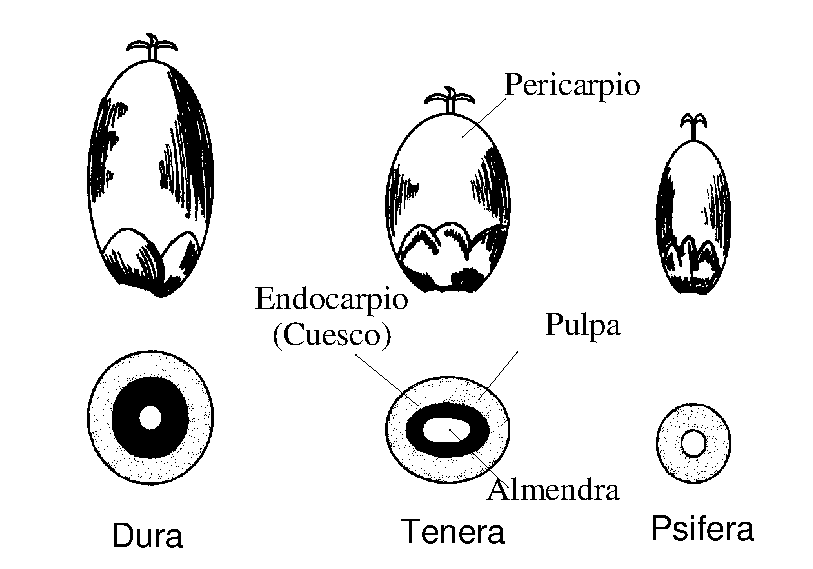
\includegraphics{Kap3/FrutoSp}%
\caption{Tipos y partes del fruto de palma de aceite \cite{AG03p,AG04p}.} \label{fig:Fruto}
\end{figure}

\section{Ejemplo de presentaci\'{o}n y citaci\'{o}n de tablas y cuadros}
Para la edici\'{o}n de tablas, cada columna debe llevar su t\'{\i}tulo; la primera palabra se debe escribir con may\'{u}scula inicial y preferiblemente sin abreviaturas. En las tablas y cuadros, los t\'{\i}tulos y datos se deben ubicar entre l\'{\i}neas horizontales y verticales cerradas (como se realiza en esta plantilla).\\

La numeraci\'{o}n de las tablas se realiza de la misma manera que las figuras o ilustraciones, a lo largo de todo el texto. Deben llevar un t\'{\i}tulo breve, que concreta el contenido de la tabla; \'{e}ste se debe escribir en la parte superior de la misma. Para la presentaci\'{o}n de cuadros, se deben seguir las indicaciones dadas para las tablas.\\

Un ejemplo para la presentaci\'{o}n y citaci\'{o}n de tablas (citaci\'{o}n indirecta), se presenta a continuaci\'{o}n:\\

De esta participaci\'{o}n aproximadamente el 60 \% proviene de biomasa
(Tabla \ref{EMundo1}).
\begin{center}
\begin{threeparttable}
\centering%
\caption{Participaci\'{o}n de las energ\'{\i}as renovables en el suministro
total de energ\'{\i}a primaria \cite{AG02i}.}\label{EMundo1}
\begin{tabular}{|l|c|c|}\hline
&\multicolumn{2}{c|}{Participaci\'{o}n en el suministro de energ\'{\i}a primaria /\% (Mtoe)\;$\tnote{1}$}\\\cline{2-3}%
\arr{Region}&Energ\'{\i}as renovables &Participaci\'{o}n de la biomasa\\\hline%
Latinoam\'{e}rica&28,9 (140)&62,4 (87,4)\\\hline%
\:Colombia&27,7 (7,6)&54,4 (4,1)\\\hline%
Alemania&3,8 (13,2)&65,8 (8,7)\\\hline%
Mundial&13,1 (1404,0)&79,4 (1114,8)\\\hline
\end{tabular}
\begin{tablenotes}
\item[1] \footnotesize{1 kg oe=10000 kcal=41,868 MJ}
\end{tablenotes}
\end{threeparttable}
\end{center}

NOTA: en el caso en que el contenido de la tabla o cuadro sea muy extenso, se puede cambiar el tama\~{n}o de la letra, siempre y cuando \'{e}sta sea visible por el lector.\\

\subsection{Consideraciones adicionales para el manejo de figuras y tablas}
Cuando una tabla, cuadro o figura ocupa m\'{a}s de una p\'{a}gina, se debe repetir su identificaci\'{o}n num\'{e}rica, seguida por la palabra continuaci\'{o}n.\\

Adicionalmente los encabezados de las columnas se deben repetir en todas las p\'{a}ginas despu\'{e}s de la primera.\\

Los anteriores lineamientos se contemplan en la presente plantilla.\\

\begin{itemize}
\item Presentaci\'{o}n y citaci\'{o}n de ecuaciones.
\end{itemize}

La citaci\'{o}n de ecuaciones, en caso que se presenten, debe hacerse como lo sugiere esta plantilla. Todas las ecuaciones deben estar numeradas y citadas detro del texto.\\

Para el manejo de cifras se debe seleccionar la norma seg\'{u}n el \'{a}rea de conocimiento de la tesis  o trabajo de investigaci\'{o}n.\\
\chapter{Cap\'{\i}tulo 3}
Se deben incluir tantos cap\'{\i}tulos como se requieran; sin embargo, se recomienda que la tesis  o trabajo de investigaci\'{o}n tenga un m\'{\i}nimo 3 cap\'{\i}tulos y m\'{a}ximo de 6 cap\'{\i}tulos (incluyendo las conclusiones).\\
\chapter{Cap\'{\i}tulo ...}
Se deben incluir tantos cap\'{\i}tulos como se requieran; sin embargo, se recomienda que la tesis  o trabajo de investigaci\'{o}n tenga un m\'{\i}nimo 3 cap\'{\i}tulos y m\'{a}ximo de 6 cap\'{\i}tulos (incluyendo las conclusiones).\\
\chapter{Conclusiones y recomendaciones}
\section{Conclusiones}
Las conclusiones constituyen un cap\'{\i}tulo independiente y presentan, en forma l\'{o}gica, los resultados de la tesis  o trabajo de investigaci\'{o}n. Las conclusiones deben ser la respuesta a los objetivos o prop\'{o}sitos planteados. Se deben titular con la palabra conclusiones en el mismo formato de los t\'{\i}tulos de los cap\'{\i}tulos anteriores (T\'{\i}tulos primer nivel), precedida por el numeral correspondiente (seg\'{u}n la presente plantilla).\\

\section{Recomendaciones}
Se presentan como una serie de aspectos que se podr\'{\i}an realizar en un futuro para emprender investigaciones similares o fortalecer la investigaci\'{o}n realizada. Deben contemplar las perspectivas de la investigaci\'{o}n, las cuales son sugerencias, proyecciones o alternativas que se presentan para modificar, cambiar o incidir sobre una situaci\'{o}n espec\'{\i}fica o una problem\'{a}tica encontrada. Pueden presentarse como un texto con caracter\'{\i}sticas argumentativas, resultado de una reflexi\'{o}n acerca de la tesis o trabajo de investigaci\'{o}n.\\
\begin{appendix}
\chapter{Anexo: Nombrar el anexo A de acuerdo con su contenido}\label{AnexoA}
Los Anexos son documentos o elementos que complementan el cuerpo de la tesis o trabajo de investigaci\'{o}n y que se relacionan, directa o indirectamente, con la investigaci\'{o}n, tales como acetatos, cd, normas, etc.\\

\chapter{Anexo: Nombrar el anexo B de acuerdo con su contenido}
A final del documento es opcional incluir \'{\i}ndices o glosarios. \'{E}stos son listas detalladas y especializadas de los t\'{e}rminos, nombres, autores, temas, etc., que aparecen en el mismo. Sirven para facilitar su localizaci\'{o}n en el texto. Los \'{\i}ndices pueden ser alfab\'{e}ticos, cronol\'{o}gicos, num\'{e}ricos, anal\'{\i}ticos, entre otros. Luego de cada palabra, t\'{e}rmino, etc., se pone coma y el n\'{u}mero de la p\'{a}gina donde aparece esta informaci\'{o}n.\\

\chapter{Anexo: Nombrar el anexo C de acuerdo con su contenido}
MANEJO DE LA BIBLIOGRAF\'{I}A: la bibliograf\'{\i}a es la relaci\'{o}n de las fuentes documentales consultadas por el investigador para sustentar sus trabajos. Su inclusi\'{o}n es obligatoria en todo trabajo de investigaci\'{o}n. Cada referencia bibliogr\'{a}fica se inicia contra el margen izquierdo.\\

La NTC 5613 establece los requisitos para la presentaci\'{o}n de referencias bibliogr\'{a}ficas citas y notas de pie de p\'{a}gina. Sin embargo, se tiene la libertad de usar cualquier norma bibliogr\'{a}fica de acuerdo con lo acostumbrado por cada disciplina del conocimiento. En esta medida es necesario que la norma seleccionada se aplique con rigurosidad.\\

Es necesario tener en cuenta que la norma ISO 690:1987 (en Espa\~{n}a, UNE 50-104-94) es el marco internacional que da las pautas m\'{\i}nimas para las citas bibliogr\'{a}ficas de documentos impresos y publicados. A continuaci\'{o}n se lista algunas instituciones que brindan par\'{a}metros para el manejo de las referencias bibliogr\'{a}ficas:\\

\begin{center}
\centering%
\begin{tabular}{|p {7.5 cm}|p {7.5 cm}|}\hline
\arr{Instituci\'{o}n}&Disciplina de aplicaci\'{o}n\\\hline%
Modern Language Association (MLA)&Literatura, artes y humanidades\\\hline%
American Psychological Association (APA)&Ambito de la salud (psicolog\'{\i}a, medicina) y en general en todas las ciencias sociales\\\hline
Universidad de Chicago/Turabian &Periodismo, historia y humanidades.\\\hline
AMA (Asociaci\'{o}n M\'{e}dica de los Estados Unidos)&Ambito de la salud (psicolog\'{\i}a, medicina)\\\hline
Vancouver &Todas las disciplinas\\\hline
Council of Science Editors (CSE)&En la actualidad abarca diversas ciencias\\\hline
National Library of Medicine (NLM) (Biblioteca Nacional de Medicina)&En el \'{a}mbito m\'{e}dico y, por extensi\'{o}n, en ciencias.\\\hline
Harvard System of Referencing Guide &Todas las disciplinas\\\hline
JabRef y KBibTeX &Todas las disciplinas\\\hline
\end{tabular}
\end{center}

Para incluir las referencias dentro del texto y realizar lista de la bibliograf\'{\i}a en la respectiva secci\'{o}n, puede utilizar las herramientas que Latex suministra o, revisar el instructivo desarrollado por el Sistema de Bibliotecas de la Universidad Nacional de Colombia\footnote{Ver: www.sinab.unal.edu.co}, disponible en la secci\'{o}n "Servicios", opci\'{o}n "Tr\'{a}mites" y enlace "Entrega de tesis".

\end{appendix}
\addcontentsline{toc}{chapter}{\numberline{}Bibliograf\'{\i}a}
\bibliographystyle{plaindin_esp}
\bibliography{BibliMSc}
\end{document}